\subsection{Метрика Махаланобис}
        
    \comment{Тут опиши эту метрику}

    Метрика Махаланобис расчитывается по формуле 

    \[d_M = \frac{|x_1 - x^*|}{\sqrt{M}}\]
        
    где \(x_1\) --- устойчивое равновесие, \(x^*\) --- либо неустойчивое равновесие, либо его прообраз. \(M\) --- значение функции стохастической чувствительности.

    Метрика Махаланобис показывает расстояние между двумя точками без учета того, что в модели \comment{что-то есть...}

    Графики метрик изображены на рисунках \ref{mahalanobis_metrics_alpha_noise}, \ref{mahalanobis_metrics_beta_noise} и \ref{mahalanobis_metrics_additive_noise}

    \begin{figure}
        \centering
        \subfloat[Для модели (\ref{alpha_chaos})]{
            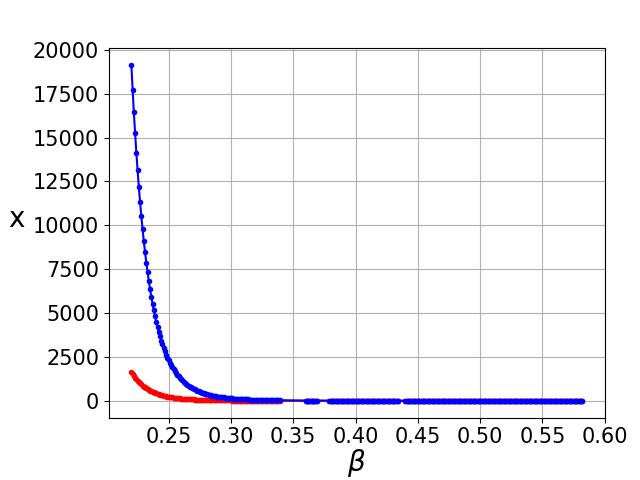
\includegraphics[width=0.55\textwidth]{stochastic/images/mahalanobis_metrics_alpha_noise.jpg}
            \label{mahalanobis_metrics_alpha_noise}
        }

        \subfloat[Для модели (\ref{beta_chaos})]{
            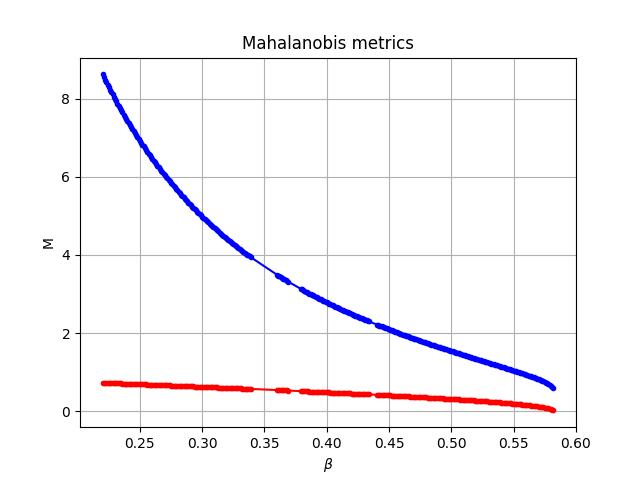
\includegraphics[width=0.55\textwidth]{stochastic/images/mahalanobis_metrics_beta_noise.jpg}
            \label{mahalanobis_metrics_beta_noise}
        }  

        \subfloat[Для модели (\ref{additive_chaos})]{
            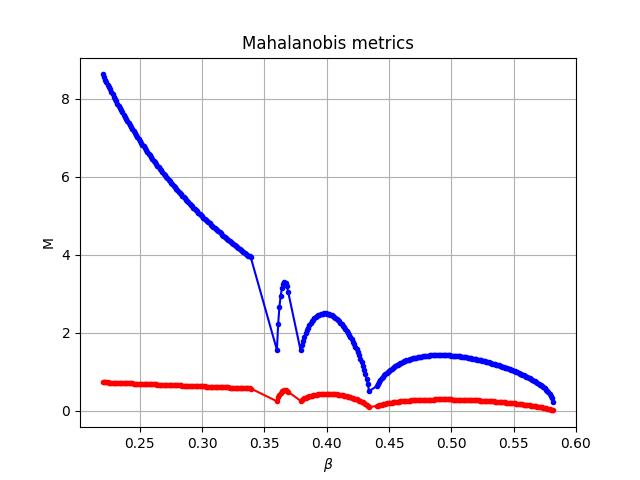
\includegraphics[width=0.55\textwidth]{stochastic/images/mahalanobis_metrics_additive_noise.jpg}
            \label{mahalanobis_metrics_additive_noise}
        }
        
        \caption{Метрика Махаланобис}
    \end{figure}
